\section{State of the art}
\label{sec:state_of_the_art}
%\subsection{\textbf{About dMRI and deterministic tractography}}
%Scientists in neuroscience seek to gain knowledge of the physical processes that underlie human sensation, attention awareness and cognition. These results are immediately applicable to surgical intervention, to the design of medical interventions and to the treatment of psychological and psychiatric disorders. However, the understanding of the brain, up to present, is currently still an uncover problem. 

%In recent years, \textbf{dMRI-Diffusion Magnetic Resonance Imaging} has gained tremendous popularity in neuro community and became one of the first methods that made it possible to visualize and quantify the organization of white matter in the human brain in vivo.
%\textbf{dMRI-Diffusion Magnetic Resonance Imaging} is evolving into a potent tool in the examination of the central nervous system. 
%Actually, it is a technique that measures local diffusivity of water within the tissue and provides information about the orientation of white matter fiber tracts.
%produces in vivo images of biological tissues by exploiting the constrained diffusion properties of water molecules. In neuroscience,
%dMRI is usually used to extract neuronal fibers from brain dMRI and it offers a good look into brain micro-structure at a scale that is not easily accessible with other modalities, in some cases improving the detection and characterization of white matter abnormalities. 
%Because of that, dMRI can help understand brain connectivity deeply, that has lead to numerous beneficial in both diagnosis and clinical applications. More 
Recently, several groups have proposed tractography methods for reconstruction the whole brain tractography from dMRI data~\cite{zhang2008identifying}. The most popular is the \textbf{deterministic tractography} algorithms~\cite{mori2002fiber}
%, by which we can reconstruct the whole brain tractography from dMRI data. and have reported success in following fiber tracts
An example of the partial tractography extracting from dMRI by using deterministic algorithm is shown in figure \ref{fig:tractography}.
%From dMRI data, the local fiber orientation distribution can be inferred and white matter fiber trajectories as a set of \emph{streamlines} can be reconstructed using the \textbf{deterministic tractography} algorithms~\cite{mori2002fiber}. 
%A \textbf{streamline} is a vectorial representation of thousands of neighboring neuronal axons sharing the same structural connectivity path. The whole set of streamlines of a brain is called \textbf{tractography} (see Figure~\ref{fig:tractography}). The resolution of modern MRI scanners is in the order of $1mm^3$, a full brain tractography consists of $\approx 3 \times 10^5$ streamlines.
\begin{figure}
  \centering
  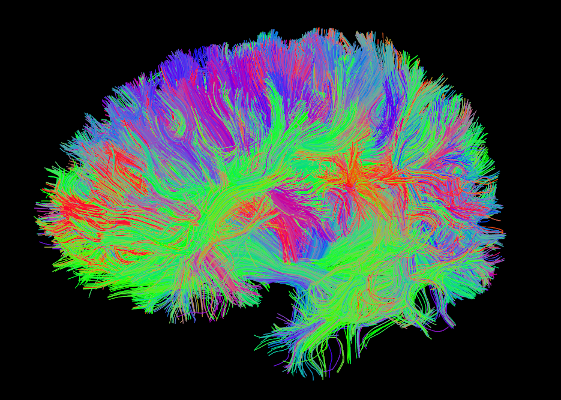
\includegraphics[width=3.18cm, height=2.2cm ]{figures/tractography.png}
  \caption{A tractography of $\approx 3\times 10^5$ streamlines within a brain. 
%(whole set of polylines) made of $\approx 3\times 10^5$ streamlines (polylines) describes the pathways of neural axons within the brain.
	Each single streamlines represents thousands of neighboring neuronal axons expressing structural connectivity.
	Only $3\%$ of the streamlines are shown to improve readability. 
	%Colors represents the main direction of each streamline.
	}
  \label{fig:tractography}
\end{figure}
%-------------------------------------------------------------------------------------------------------
%\subsection{\textbf{About Tractography segmentation}}
However, the resulting tractography datasets are highly complex and include thousands of fibers (about $\approx 3 \times 10^5$), which requires techniques or method to create the exact anatomic brain before doing further studying. The \textbf{segmentation} aims at doing this task, groups some fiber tracts belonging to a common anatomical area into one segmentation. Due to the fact that the complex tractography datasets present a large amount of short association bundles which have been rarely studied until now, it is extremely difficult to cluster some fibers having the same anatomical structure into a group. The segmentation of fiber bundles is therefore a complex and not completely solved problem. 
%Furthermore, clinical studies often use the segmentation of white matter bundles in order to perform comparisons between populations. This is also an press on the accuracy of the segmentation task. 
%The next goal is how we can group some fiber tracks which has the same function into \emph{the specific anatomically structures}. This \textbf{segmentation of the neural streamlines} is a task of interest in neurological studies, for example for the study of Alzheimer disease~\cite{bozzali2002white}. Unlike a simplistic bundle model, where known white matter tracts are represented by a relatively small number of fibers with the same shape, current tractography datasets reconstruct tracts represented by thousands of fibers, composed of various fiber fascicles of different shapes and lengths. 
%Several examples of decomposition of major fiber tracts were already proposed~\cite{lawes2008atlas}. 
%Also, these complex tractography datasets present a large amount of short association bundles, that have been rarely studied until now. Due to the large number of streamlines in a brain (about $\approx 3 \times 10^5$), it is extremely difficult to cluster some streamlines having the same anatomically structure into a group. The segmentation of fiber bundles is therefore a complex and not completely solved problem. 
Recently, the literature about machine learning techniques to solve this problem is increasing. 
%Recently, there is a rise of applying pattern recognition techniques to solve this problem. %Our goal is to applying machine learning techniques to segment the fiber bundles of the human brain. 
In the following part, the brief survey about currently trends in segmentation tractography are presented.

\textbf{\textit{Atlas approach}}
%from Elestherios 78
%To avoid the difficulty of choosing number of clusters, using atlas as prior knowledge is another approach. 
Atlas are the models of white mater structure in brain. 
%The number of clusters is already defined in this atlas, and this leads to no cluster center selection. 
Firstly, atlas are created from experience of experts without being driven from data. After that, atlas are used as model of clusters for tractography segmentation. All streamlines would be grouped into the closest cluster in atlas. O'Donnell and Westin~\cite{odonnell2007automatic} generated a tractographic atlas using spectral embedding and expert anatomical labeling. They then automatically segmented the new tractography using again spectral clustering and embedding the tracks as points in the embedded space, to the closest existing atlas clusters. The true affinity matrix was too big to compute therefore they used the Nystrom approximation: working on a subset and avoid generating the complete distance matrix. However, the important information from the full data set may be lost after sub-sampling. The other main issue of this approach is that up to present, there is no believable algorithm for co-registration two anatomical brains due to the difference of size, position, and direction of these brains.

\textbf{\textit{ROI - region of interest}}
%from Elestherios 78
One of the first idea for segmentation is to use the region of interest (ROI)~\cite{wakana2007reproducibility}. This approach tried to reconstruct tracts passing through ROI by exploiting existing anatomical knowledge of tract trajectories. First, some target tracts must be defined. It also requires to specified manually some regions where tracts start, end or pass through. Then streamlines would be filtered based on the constraint of passing through ROIs. ROI approach needs a priori knowledge about the trajectory and is used only for well-characterized white matter tracts.  
%First, tracking was performed from all pixels inside the brain (brute-force approach)~\cite{hua2008tract}. And results penetrating the manually defined ROIs were assigned to the specific tracts associated with the ROIs. 
In order to refine the segmentation, multi-ROIs were used to include or exclude tracks.
%generated by FACT and Hua et al. [67] used regions of interest together with probabilistic tractography. Zvitia et al. [159], [160] used adaptive mean shift so that they do not need to provide the number of clusters, they also used this approach for registration of datasets from the same subject.

\textbf{\textit{Unsupervised learning }}%without dissimilarity approach} %(in wang2011tractography)
From the point of view of algorithmic approaches, the segmentation task has traditionally been addressed with unsupervised techniques over only diffusion data~\cite{zhang2008identifying}. This typical framework first defines a pairwise distance between fibers and inputs the similarity matrix to standard clustering algorithms. Various distance functions between fibers have been proposed: the Euclidean distances between fiber shape descriptors~\cite{brun2004clustering}; the similarity between two fibers based on the number of points sharing the same voxel~\cite{jonasson2005fiber}; distance from the B-spline representation~\cite{maddah2005automated} ; closest point distance, mean of closest distances and Hausdorff distance~\cite{gerig2004analysis}. Then, following is a clustering algorithm (agglomerative, k-means, Gaussian mixture model, etc. see~\cite{wang2011tractography} for a recent brief review of applying these algorithm for tractography).
%Such techniques often rely on expert-crafted streamline-streamline distance functions encoding informative relationships for the segmentation task.
\\The disadvantage of these clustering algorithms is that they require manually specifying the number of clusters or a threshold for decide when to stop merging or splitting clusters. The different numbers of chosen clusters vary significantly the performance of clustering~\cite{moberts2005evaluation}. 
%In the case that the datasets are complicated and noisy, both of them are difficult to specify. 
Recently, there are some approaches try to solve this problem by auto choosing the number of clusters. In~\cite{odonnell2007automatic}, a large cluster number for spectral clustering is chosen, and then these clusters are manually merged to obtain models for white matter structures. Zvitia et al.~\cite{zvitia2008adaptive} and Wassermannet al.~\cite{wassermann2010unsupervised} decide the number of clusters based on mean-shift. %Zvitia et al.~\cite{zvitia2008adaptive} required calculating the average of fibers, which was not easy in cases when fibers were not represented as feature vectors and only fiber similarities were available. 
By adding a penalty to a larger cluster number, Neji et al.~\cite{neji2009clustering} solved the optimization using linear programming to chose the number of clusters. Recently, Garyfallidis et al.~\cite{garyfallidis2012quickbundles} proposed a very quick clustering algorithm, called QuickBundles. It took one random streamlines as initial cluster, and calculated the distance from all the un-clustered streamlines to the representatives of clusters. Only the streamline with the minimum distance was grouped into the closest cluster if the distance was less than a given threshold, other while, that streamline became a new cluster. 
\\Although these approaches avoid manually choosing number of cluster, the drawback is the high space and time complexities of computing pairwise distances between fibers. Whole brain tractography produces $\approx 3 \times 10^5$ streamlines fibers per subject, it is difficult to compute, and it becomes more serious when clustering fibers of multiple subjects. To avoid computing pairwise distances between fibers, Savadjiev et. al.~\cite{savadjiev2008streamline} clustered diffusion orientation distribution functions maxima instead of clustering fiber tracts directly. This algorithm based on the geometric coherence of fiber orientations. Maddah et al. in~\cite{maddah2008modeling} proposed a probabilistic approach to cluster fibers. It used a Dirichlet distribution as a prior to incorporate anatomical information. However, this algorithm also required establishing point correspondence which was difficult to define. 
\\The most disadvantage of unsupervised approach is that it works on the whole tractogrpahy and tries to cluster tractography into many tracts. While the requirement of medical practitioners only focuses on some specific tracts.   
%Besides this framework, some other approaches have been proposed in recent years.
%In~\cite{savadjiev2008streamline}, Savadjiev et. al clustered diffusion orientation distribution functions maxima instead of clustering fiber tracts directly. This algorithm based on the geometric coherence of fiber orientations. Maddah et al. in~\cite{maddah2008modeling} proposed a probabilistic approach to cluster fibers. There was no need to computing pairwise distances in this approach, because it used a Dirichlet distribution as a prior to incorporate anatomical information. This algorithm also required establishing point correspondence which was difficult to define. Wang et al.~\cite{wang2011tractography} proposed a non-parametric Bayesian framework to cluster white matter fiber tracts into bundles using a hierarchical Dirichlet processes mixture (HDPM) model. %After the models of bundles is learned from training data without supervision, they can be used as prior to cluster fibers of new subjects for comparison across subjects.
%The current solutions are to cluster only a small portion of the whole data set after subsampling or to do some numerical approximation based on the sampled subset (O'Donnell and Westin, 2007). However, important information from the full data set may be lost after subsampling. 
%Then later in [110] they tried group analysis on prespecified bundles.
%To avoid this difficulity, using atlas as prior knowledge is another approach. This atlas is the model of white mater structure in brain. The number of clusters is already defined in this atlas, and this leads to no cluster center selection. There are many way to choose this number. In~\cite{odonnel2007automatic}, a large cluster number for spectral clustering is chosen, and then these clusters are manually merged to obtain models for white matter structures. Zvitia et al.~\cite{zvitia2008adaptive} and Wassermannet al.~\cite{wassermann2010unsupervised} decide the number of clusters based on mean-shift. Zvitia et al.~\cite{zvitia2008adaptive} required calculating the average of fibers, which was not easy in cases when fibers were not represented as feature vectors and only fiber similarities were available. By adding a penalty to a larger cluster number, Neji et al.~\cite{neji2009clustering} solving the optimization using linear programming to chose the number of clusters. Although this approach avoids manually choosing number of cluster, the drawback of this framework is the high space and time complexities of computing pairwise distances between fibers when the data set is large. Whole brain tractography produces $\approx 3 \times 10^5$ streamlines fibers per subject, it is difficult to compute. This problem becomes more serious when clustering fibers of multiple subjects. 
%The current solutions are to cluster only a small portion of the whole data set after subsampling or to do some numerical approximation based on the sampled subset \cite{Odonnell2007automatic}. However, important information from the full data set may be lost after subsampling.

\textbf{\textit{Supervised learning}}
Supervised segmentation is the method of partitioning according to provided examples. 
Firstly, the target tracts should be specific, such as corticol spinal tracts (see figure~\ref{fig:CST}. Then, a repository of samples must be collected. A sample is an expert-made assignment of streamlines to the target tracts. These samples are used to train a classify model, which is used to cluster a new streamline. In this setting, each streamline can be class-labelled as being member of the fiber tract of interest or not. For this reason the supervised segmentation problem becomes a binary classification problem. 
\\Up to present, there is a little attention in the literature about supervised tract segmentation.
Maddah et al.~\cite{maddah2005automated} used the $B$-spline representation of the streamlines, and classified by the nearest-neighbor algorithm with respect to an atlas. 
In~\cite{odonnell2007automatic}, O'donnel created an atlas from training dataset based on spectral clustering. 
%and the most recent on hierarchical Dirichlet processes~\cite{wang2011tractography}. 
Wang et al.~\cite{wang2011tractography} proposed a non-parametric Bayesian framework using a hierarchical Dirichlet processes mixture (HDPM) model. %After the models of bundles is learned from training data without supervision, they can be used as prior to cluster fibers of new subjects for comparison across subjects.
The models of bundles were learned from how voxels are connected by fibers in training data instead of comparing fiber distances. Olivetti~\cite{olivetti2010brain} combined both structural and functional connectivity to study jointly in a pairwise approach with the goal of assessing the contributions of structural information and functional information when segmenting the tracts. Recently,~\cite{olivetti2011supervised} solved this classification problem basing on the dissimilarity representation. After projecting all streamlines into some prototypes, one streamline-streamline distance function is computed in this new representation space, and it is used for classifying.
\\Although supervised approaches focus on a specific tracts as requirement of medical practitioners. %These approaches get some encouragement results. 
However,
%they need to be refined by medical practitioners to be used in clinical applications. Another issue is that
because the number of data for training and testing is very small due to the vague time for collecting enough the truth background data of manual segmentation tractography, the results usually are bellow the expectation of medical practitioners, and they need to be refined to use in clinical applications.
%Supervised tract segmentation instead aims at learning how to segment the tractography from expert-made examples provided as input. Up to present, there is a little attention in the literature about supervised tract segmentation.
%Supervised tract segmentation instead aims at learning how to segment the tractography from expert-made examples provided as input. Supervised tract segmentation has received little attention so far in the literature. To the best of our knowledge only a few different approaches have been proposed. 
%Segmenting a given tractography is the task of partitioning it into subsets of streamlines. \emph{Supervised} segmentation is the task of partitioning according to provided examples. An example is an expert-made assignment of streamlines to categories of interest, like neuroanatomic fiber tracts. Supervised segmentation uses examples to guide the segmentation of further tractography data. In this work we restrict the segmentation task to segmenting a single specific fiber tract of interest at a time and we assume to have available examples. In this setting each streamline can be class-labeled as being member of the fiber tract of interest or not. For this reason the supervised segmentation problem becomes a binary classification problem.
%\textbf{\textit{Dirichlet distribution approach}} %(in wang2011tractography)
%Besides these framework, in recently, some other approaches have been proposed for this segmentation task.
%% (Maddah et al., 2008b; Savajiev et al., 2008; Wassermann et al., 2009; Wassermann et al., 2010). 
%A fiber tract segmentation algorithm based on the geometric coherence of fiber orientations is proposed in~\cite{savadjiev2008streamline}. This method clusters diffusion orientation distribution functions maxima instead of clustering fiber tracts directly. Maddah et al. in~\cite{maddah2008modeling} proposed a probabilistic approach to cluster fibers. There is no need to computing pairwise distances in this approach, because it uses a Dirichlet distribution as a prior to incorporate anatomical information. It used a parametric model, assuming that the number of clusters is known and required manual initialization of cluster centers. This algorithm also required establishing point correspondence which was difficult to define. 
%Wang et al.~\cite{wang2011tractography} overcomes these obstacles by proposing a non-parametric Bayesian framework to cluster white matter fiber tracts into bundles using a hierarchical Dirichlet processes mixture (HDPM) model. After the models of bundles is learned from training data without supervision, they can be used as prior to cluster fibers of new subjects for comparison across subjects. Although this approach does not require computing pairwise distances between fibers, but the number of clusters must be specified prior manually or automatically.

%\subsection{\textbf{What we propose}}
\begin{figure*}
  \centering
  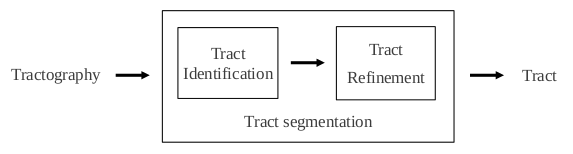
\includegraphics[width=12.5cm, height=2.5cm ]{figures/segmentation.png}
  \caption{A process design of segmentation task, including two steps: tract identification and tract refinement. The tract identification creates the candidate of segmentation from a repository of examples using a supervised algorithm. The candidate then will be refined by experts with the help of the fast clustering technique.}
  \label{fig:ov_tool}
\end{figure*}
The drawback of these approaches is that or they work on a large number of tracks and most of them are not interested to medical practitioners; or they focus on a target tract but the variance between brains makes it difficult to generate well. The results from both case are needed the refinement from expert. In this work, we want to combine both supervised and unsupervised approach to overcome these disadvantage. Moreover, we propose a framework using \textbf{BOI}(Bundles of Interest). While ROI concerns about which streamlines go through some interesting regions, BOI focuses only on streamlines inside some specific bundles. Because all of the current approaches only work on the tracks without caring the anatomy,
% (for example\cite{wakana2007reproducibility} based on ROI-region of interest,~\cite{odonnell2007automatic} needed an Atlas),
and it makes difficult to validate the result. Using BOI would make medical practitioners concentrate on which tracts they are working on, and of course these tracts also correlate to the anatomy. Moreover, while all the current methods are off-line and medical practitioners can not interact or modify the result of segmentation, in this project, we want to build a tool that can help them instantly to refine the segmentation result mannualy. It is also another novelty of our approach. Beside, this tool should has ability of real time adapting to the responding of users. This is also the other different of our method to most of the state-of-the-art approaches, which can not adjust to the user feedback. In another way, in this project, our goals are to:
%The most challenge is to design a clustering algorithm based on a specific distance function and this algorithm must be effective and real time adaptive to the responding of users. This is also the other different of our method to most of the state-of-the-art approaches, which can not adjust to the user feedback.
%In this project, our goal is to address the segmentation problem based on the BOI (Bundle of Interest) contrasting with ROI (Region of Interest). : 
%What is the outline of research?
\begin{itemize}
	\item First, design an effective method for tract segmentation task using \emph{machine learning} based on BOI approach.
%techniques
	\item Second, develop a scientific interactive visualization tool, which is the implementation of the framework that we propose for tract segmentation task in the previous step.%in the first goal, to help medical practitioners to perform this segmentation task more precisely and easily based on BOI approach.
\end{itemize}
With the assistance of this scientific interactive tool, we have a strong belief that the task of tract segmentation would be done more precisely, more easily and would consume less time.
%This research is motivated to help medical practitioners to do the task of segmentation tractography more easily and accurately. Results of tract segmentation are immediately applicable to surgical intervention, to the design of medical interventions and to the treatment of psychological and psychiatric disorders. The end users who got benefit from this work are patients who have problem with their brain or other cognitive issues.
%We propose a design of interactive segmentation process based on two steps: tract identification 
%based on supervised learning 
%and tract refinement (figure \ref{fig:ov_tool}).
%with the help from unsupervised learning. 
%The tract identification step generates the first hypothesis of segmentation instead of starting from the whole tractography. This step uses the manual segmentation examples from experts to create the candidate of tract segmentation, and we conceive it as a supervised learning task. This step can be solved based on the most recent method introduced in% by Olivetti
%~\cite{olivetti2011supervised}. The next refinement step aims to refine the hypothesis of segmentation and takes place by excluding some unnecessary streamlines or selecting additional ones. With the aim to help medical practitioners to perform this refinement task more precisely and easily, it is necessary to cluster streamlines with similar spatial and shape characteristics into one set, called \emph{bundle}. We design it as a clustering problem, and our main investigation focuses on it.
%In this work we propose to address the \textbf{online segmentation task} by using both \textbf{supervised and unsupervised segmentation} (fast clustering technique). For better using and supporting doctors/neural scientists to do the segmentation task more easy and faster, we build up an interaction visualization tool, call Spaghetti. In this software, there are two main steps: the first step uses supervised learning to make the candidate of segmentation from the repository of examples. Then, doctors/neural scientists will refine this candidate in the next step with the help from fast clustering technique. The frame work of this software is described in the figure \ref{fig:ov_tool}. After the segmentation task, the result is then used for some clinical diagnosis applications.
%In this work we propose to address the segmentation tractography task as both unsupervised and supervised segmentation problem based on dissimilarity approximation. 
%Brain connectivity analysis methods – joint modeling of structural and functional brain connectivity, relationship between structural and functional connectivity, and dynamics of connectivity. more infor at http://mbia2012.web.unc.edu/
%Another one is leverage the expert-crafted streamline-streamline distance functions available from the literature and to use them in a dissimilarity based~\cite{pekalska2002generalized} representation of the problem. It means that instead of working directly to tractography dataset as these past approaches, we try to propose a new representation space for the tractography based on dissimilarity approximation. Moreover we note that the widely adopted kernel-based classification algorithms cannot directly embed such distance functions into a kernel because the kernel would violate the necessary assumption of being positive semi-definite~\cite{pekalska2002generalized,chen2009similarity}. Due to that, it is necessary to vectorize the tractography in the standard space before applying current novel learning techniques to segment. We believe that with this vectorizing, the segmentation tractography task using both unsupervised and supervised learning will get the novel results.
%of\footnote{A fourth, and last, footnote.}





